% !TeX program = lualatex
% ALIUS Bulletin native visual reconstruction source.
% Generated from off-repo reference layout data; does not include or input a pre-existing article PDF.
\ifdefined\ALIUSIssueBuild
\else
\documentclass{article}
\usepackage[paperwidth=595.0000bp,paperheight=842.0000bp,margin=0bp]{geometry}
\usepackage{graphicx}
\usepackage{xcolor}
\usepackage{tikz}
\usepackage{iftex}
\ifPDFTeX
  \usepackage[T1]{fontenc}
  \usepackage[utf8]{inputenc}
  \usepackage{textcomp}
  \usepackage{amssymb}
\else
  \usepackage{fontspec}
\fi
\pagestyle{empty}
\fi
\ifPDFTeX
  \providecommand{\ALIUSDeclareUnicodeFallbacks}{%
    \DeclareUnicodeCharacter{00AC}{\ensuremath{\neg}}%
    \DeclareUnicodeCharacter{00BE}{\ensuremath{\frac{3}{4}}}%
    \DeclareUnicodeCharacter{0101}{\=a}%
    \DeclareUnicodeCharacter{0107}{\'c}%
    \DeclareUnicodeCharacter{012B}{\=\i}%
    \DeclareUnicodeCharacter{0131}{\i}%
    \DeclareUnicodeCharacter{0142}{\l}%
    \DeclareUnicodeCharacter{015B}{\'s}%
    \DeclareUnicodeCharacter{016B}{\=u}%
    \DeclareUnicodeCharacter{025C}{q}%
    \DeclareUnicodeCharacter{0278}{t}%
    \DeclareUnicodeCharacter{02AE}{Th}%
    \DeclareUnicodeCharacter{02B0}{ff}%
    \DeclareUnicodeCharacter{02B4}{ffi}%
    \DeclareUnicodeCharacter{02BE}{ft}%
    \DeclareUnicodeCharacter{02BF}{fi}%
    \DeclareUnicodeCharacter{02C0}{fl}%
    \DeclareUnicodeCharacter{02C1}{fi}%
    \DeclareUnicodeCharacter{02D9}{Th}%
    \DeclareUnicodeCharacter{02EF}{gy}%
    \DeclareUnicodeCharacter{0394}{\ensuremath{\Delta}}%
    \DeclareUnicodeCharacter{03B2}{\ensuremath{\beta}}%
    \DeclareUnicodeCharacter{03BA}{\ensuremath{\kappa}}%
    \DeclareUnicodeCharacter{068D}{-}%
    \DeclareUnicodeCharacter{08BC}{ti}%
    \DeclareUnicodeCharacter{099E}{ti}%
    \DeclareUnicodeCharacter{1E43}{\d{m}}%
    \DeclareUnicodeCharacter{1E47}{\d{n}}%
    \DeclareUnicodeCharacter{1E63}{\d{s}}%
    \DeclareUnicodeCharacter{201C}{``}%
    \DeclareUnicodeCharacter{201D}{''}%
    \DeclareUnicodeCharacter{2260}{\ensuremath{\neq}}%
    \DeclareUnicodeCharacter{25A1}{\ensuremath{\square}}%
  }%
  \ifdefined\ALIUSIssueBuild\else\ALIUSDeclareUnicodeFallbacks\fi
  \providecommand{\ALIUSFontLatoLight}{\fontfamily{lato-LF}\fontseries{l}\selectfont}
  \providecommand{\ALIUSFontLatoRegular}{\fontfamily{lato-LF}\fontseries{m}\selectfont}
  \providecommand{\ALIUSFontLatoItalic}{\fontfamily{lato-LF}\fontseries{m}\itshape}
  \providecommand{\ALIUSFontLatoLightItalic}{\fontfamily{lato-LF}\fontseries{l}\itshape}
  \providecommand{\ALIUSFontCormorantRegular}{\fontfamily{CormorantGaramond-LF}\fontseries{m}\selectfont}
  \providecommand{\ALIUSFontCormorantLight}{\fontfamily{CormorantGaramond-LF}\fontseries{l}\selectfont}
  \providecommand{\ALIUSFontCormorantMedium}{\fontfamily{CormorantGaramond-LF}\fontseries{medium}\selectfont}
  \providecommand{\ALIUSFontCormorantBold}{\fontfamily{CormorantGaramond-LF}\fontseries{b}\selectfont}
  \providecommand{\ALIUSFontCormorantItalic}{\fontfamily{CormorantGaramond-LF}\fontseries{m}\itshape}
  \providecommand{\ALIUSFontTimes}{\fontfamily{ptm}\selectfont}
  \providecommand{\ALIUSFontCalibri}{\fontfamily{phv}\selectfont}
  \providecommand{\ALIUSFontCambria}{\fontfamily{ptm}\selectfont}
  \providecommand{\ALIUSFontSymbolFallback}{\fontfamily{ptm}\selectfont}
\else
  \providecommand{\ALIUSFontLatoLight}{\fontspec{Lato Light}}
  \providecommand{\ALIUSFontLatoRegular}{\fontspec{Lato Regular}}
  \providecommand{\ALIUSFontLatoItalic}{\fontspec{Lato Italic}}
  \providecommand{\ALIUSFontLatoLightItalic}{\fontspec{Lato Light Italic}}
  \providecommand{\ALIUSFontCormorantRegular}{\fontspec{Cormorant Garamond Regular}}
  \providecommand{\ALIUSFontCormorantLight}{\fontspec{Cormorant Garamond Light}}
  \providecommand{\ALIUSFontCormorantMedium}{\fontspec{Cormorant Garamond Medium}}
  \providecommand{\ALIUSFontCormorantBold}{\fontspec{Cormorant Garamond Bold}}
  \providecommand{\ALIUSFontCormorantItalic}{\fontspec{Cormorant Garamond Italic}}
  \providecommand{\ALIUSFontTimes}{\fontspec{Times New Roman}}
  \providecommand{\ALIUSFontCalibri}{\fontspec{Calibri}}
  \providecommand{\ALIUSFontCambria}{\fontspec{Cambria}}
  \providecommand{\ALIUSFontSymbolFallback}{\fontspec{Times New Roman}}
\fi
\definecolor{ALIUSC000000}{HTML}{000000}
\definecolor{ALIUSC1F8135}{HTML}{1F8135}
\definecolor{ALIUSC222222}{HTML}{222222}
\definecolor{ALIUSC595959}{HTML}{595959}
\definecolor{ALIUSC767171}{HTML}{767171}
\definecolor{ALIUSC7F7F7F}{HTML}{7F7F7F}
\definecolor{ALIUSCBFBFBF}{HTML}{BFBFBF}
\definecolor{ALIUSCFFFFFF}{HTML}{FFFFFF}
\providecommand{\ALIUSPlacedText}[6]{%
  \node[anchor=north west,inner sep=0pt,outer sep=0pt,text=#4] at (#1bp,-#2bp) {%
    \resizebox{#3bp}{!}{{#5\fontsize{#6bp}{#6bp}\selectfont #6\kern0pt}}%
  };%
}
\providecommand{\ALIUSPlacedTextContent}[7]{%
  \node[anchor=north west,inner sep=0pt,outer sep=0pt,text=#4] at (#1bp,-#2bp) {%
    \resizebox{#3bp}{!}{{#5\fontsize{#6bp}{#6bp}\selectfont #7}}%
  };%
}

% --- Draft abstract retained as comments; not rendered in reconstruction. ---
% \section*{Abstract}
% This interview with Simon McCarthy-Jones surveys interdisciplinary approaches to voice-hearing across terminology, psychology, history, and ethics. McCarthy-Jones explains why he favours "voice-hearing" over "auditory verbal hallucination", presenting the choice as bound up with questions of dispossession, colonization, and the right of those who hear voices to define their own experience, while acknowledging that some find the medical term useful. The conversation moves to the inner speech model developed in part with Charles Fernyhough, drawing on Lev Vygotsky's account of inner speech as a means of self-regulation, and reviews empirical tests including subvocal throat activity studies and the prospect of decoding inner speech from neural signals, alongside therapeutic uses centred on shame and Compassion Focussed Therapy. McCarthy-Jones then defends a historical perspective on voice-hearing as serving three functions: enriching phenomenology through neglected cases such as soundless voices, distinguishing culturally malleable features like command content from stable ones, and exposing the contingent reasons for the dominance of biomedical models, including political pressures from the Church of England, Andrew Scull's account of early psychiatry, and asymmetric scrutiny of trauma-based versus biological models. Further sections argue that distal causes such as trauma are not a simple addition to neuroscience and that decontextualized neural findings risk misdirecting intervention, balanced against cases like metachromatic leukodystrophy where biological analysis is informative. The interview closes on the ethical orientation of the field, distinguishing "turning away" and "turning toward" recovery stances and emphasizing collaborative research with the Hearing Voices Movement.\par
% --- End draft abstract. ---

\ifdefined\ALIUSIssueBuild
\else
\begin{document}
\fi

% Page 1
\thispagestyle{empty}
\noindent\begin{tikzpicture}[remember picture,overlay,x=1bp,y=1bp,shift={(current page.north west)}]
  \fill[ALIUSC767171] (69.640bp,-787.000bp) rectangle ++(456.480bp,-0.720bp);
  \fill[ALIUSC1F8135] (346.120bp,-166.120bp) rectangle ++(60.720bp,-0.240bp);
  \fill[ALIUSC1F8135] (346.120bp,-241.720bp) rectangle ++(166.560bp,-0.240bp);
  \fill[ALIUSCBFBFBF] (340.360bp,-136.600bp) rectangle ++(0.240bp,-82.080bp);
  \fill[ALIUSCBFBFBF] (340.360bp,-218.680bp) rectangle ++(0.240bp,-2.160bp);
  \fill[ALIUSCBFBFBF] (340.360bp,-220.840bp) rectangle ++(0.240bp,-48.240bp);
  \ALIUSPlacedTextContent{511.620}{35.460}{14.844}{ALIUSC767171}{\ALIUSFontLatoLight}{10.800}{37}
  \ALIUSPlacedTextContent{71.080}{71.099}{305.181}{ALIUSC000000}{\ALIUSFontLatoRegular}{19.920}{The phenomenon of voice-hearing}
  \ALIUSPlacedTextContent{71.080}{101.311}{227.013}{ALIUSC000000}{\ALIUSFontLatoLight}{17.755}{An interdisciplinary approach}
  \ALIUSPlacedTextContent{74.920}{136.566}{125.486}{ALIUSC000000}{\ALIUSFontLatoLight}{15.840}{An interview with}
  \ALIUSPlacedTextContent{346.120}{141.316}{124.665}{ALIUSC000000}{\ALIUSFontLatoRegular}{12.000}{Simon McCarthy-Jones}
  \ALIUSPlacedTextContent{74.920}{155.807}{193.192}{ALIUSC000000}{\ALIUSFontLatoLight}{18.960}{Simon McCarthy-Jones}
  \ALIUSPlacedTextContent{346.120}{156.155}{64.092}{ALIUSC1F8135}{\ALIUSFontLatoLight}{8.880}{mccartsi@tcd.ie}
  \ALIUSPlacedTextContent{346.120}{166.955}{102.178}{ALIUSC000000}{\ALIUSFontLatoLight}{8.880}{Department of Psychiatry}
  \ALIUSPlacedTextContent{346.120}{177.755}{118.188}{ALIUSC000000}{\ALIUSFontLatoLight}{8.880}{Trinity College, Dublin, Ireland}
  \ALIUSPlacedTextContent{74.920}{190.528}{130.282}{ALIUSC000000}{\ALIUSFontLatoLight}{12.960}{By Mathieu Frerejouan}
  \ALIUSPlacedTextContent{346.120}{216.916}{107.122}{ALIUSC000000}{\ALIUSFontLatoRegular}{12.000}{Mathieu Frerejouan}
  \ALIUSPlacedTextContent{74.920}{221.208}{262.198}{ALIUSC000000}{\ALIUSFontLatoLight}{9.840}{Citation: McCarthy-Jones, S., \& Frerejouan, M. (2017). The}
  \ALIUSPlacedTextContent{346.120}{231.755}{169.911}{ALIUSC1F8135}{\ALIUSFontLatoLight}{8.880}{mathieu.frerejouan-du-saint@univ-paris1.fr}
  \ALIUSPlacedTextContent{74.920}{233.208}{262.199}{ALIUSC000000}{\ALIUSFontLatoLight}{9.840}{phenomenon of voice-hearing: an interdisciplinary approach.}
  \ALIUSPlacedTextContent{346.120}{242.555}{102.363}{ALIUSC000000}{\ALIUSFontLatoLight}{8.880}{Department of Philosophy}
  \ALIUSPlacedTextContent{74.920}{245.208}{186.409}{ALIUSC000000}{\ALIUSFontLatoLight}{9.840}{An interview with Simon McCarthy-Jones.}
  \ALIUSPlacedTextContent{262.925}{245.208}{58.969}{ALIUSC000000}{\ALIUSFontLatoLightItalic}{9.840}{ALIUS Bulletin}
  \ALIUSPlacedTextContent{321.975}{245.208}{3.874}{ALIUSC000000}{\ALIUSFontLatoLight}{9.840}{,}
  \ALIUSPlacedTextContent{327.445}{245.208}{5.707}{ALIUSC000000}{\ALIUSFontLatoLightItalic}{9.840}{1}
  \ALIUSPlacedTextContent{333.245}{245.208}{3.874}{ALIUSC000000}{\ALIUSFontLatoLight}{9.840}{,}
  \ALIUSPlacedTextContent{346.120}{253.355}{173.461}{ALIUSC000000}{\ALIUSFontLatoLight}{8.880}{Pantheon-Sorbonne University, Paris, France}
  \ALIUSPlacedTextContent{74.920}{257.208}{26.431}{ALIUSC000000}{\ALIUSFontLatoLight}{9.840}{37-45}
  \ALIUSPlacedTextContent{71.080}{317.167}{455.712}{ALIUSC1F8135}{\ALIUSFontLatoLight}{12.310}{First of all, you usually define your object of study as "voice-hearing" rather than}
  \ALIUSPlacedTextContent{71.080}{334.447}{455.709}{ALIUSC1F8135}{\ALIUSFontLatoLight}{12.310}{"auditory verbal hallucinations." Can you tell us why this distinction is essential for you?}
  \ALIUSPlacedTextContent{71.080}{363.498}{456.459}{ALIUSC000000}{\ALIUSFontCormorantRegular}{13.920}{The distinction is important to me because it is important to a lot of people who}
  \ALIUSPlacedTextContent{71.080}{380.538}{456.596}{ALIUSC000000}{\ALIUSFontCormorantRegular}{13.920}{hear voices. For someone new to the field, this might seem like a fairly dry}
  \ALIUSPlacedTextContent{71.080}{397.338}{456.561}{ALIUSC000000}{\ALIUSFontCormorantRegular}{13.920}{terminological debate. It is not. Many have argued that it is part of a wider problem}
  \ALIUSPlacedTextContent{71.080}{414.378}{456.601}{ALIUSC000000}{\ALIUSFontCormorantRegular}{13.920}{of dispossession, imposition, and colonization. This problem is set out well in a}
  \ALIUSPlacedTextContent{71.080}{431.178}{85.712}{ALIUSC000000}{\ALIUSFontCormorantRegular}{13.920}{paper entitled "}
  \ALIUSPlacedTextContent{156.829}{431.178}{112.460}{ALIUSC000000}{\ALIUSFontCormorantItalic}{13.920}{Reclaiming Experience}
  \ALIUSPlacedTextContent{269.358}{431.178}{258.293}{ALIUSC000000}{\ALIUSFontCormorantRegular}{13.920}{" by Jacqui Dillon and Rufus May (2003), both}
  \ALIUSPlacedTextContent{71.080}{448.218}{456.578}{ALIUSC000000}{\ALIUSFontCormorantRegular}{13.920}{of whom have been the recipients of psychiatric treatment. In this, they stress their}
  \ALIUSPlacedTextContent{71.080}{465.258}{456.537}{ALIUSC000000}{\ALIUSFontCormorantRegular}{13.920}{right to "define ourselves" and to "find our own voice to describe our experiences}
  \ALIUSPlacedTextContent{71.080}{482.058}{456.565}{ALIUSC000000}{\ALIUSFontCormorantRegular}{13.920}{and our lives". You can see the potential benefit of this in something my colleague}
  \ALIUSPlacedTextContent{71.080}{499.098}{390.989}{ALIUSC000000}{\ALIUSFontCormorantRegular}{13.920}{Amanda Waegeli (2013) wrote about her own voice-hearing experiences:}
  \ALIUSPlacedTextContent{99.430}{528.232}{399.422}{ALIUSC000000}{\ALIUSFontCormorantRegular}{12.000}{Psychiatry, professionals and academics… will all put their own interpretations on my}
  \ALIUSPlacedTextContent{99.430}{542.632}{399.422}{ALIUSC000000}{\ALIUSFontCormorantRegular}{12.000}{experience and explain it in whatever way they like to, but the bottom line is it doesn't}
  \ALIUSPlacedTextContent{99.430}{557.272}{399.411}{ALIUSC000000}{\ALIUSFontCormorantRegular}{12.000}{matter to me anymore now what they think. I accept my voice hearing experiences as}
  \ALIUSPlacedTextContent{99.430}{571.672}{399.414}{ALIUSC000000}{\ALIUSFontCormorantRegular}{12.000}{being normal for me. I once wanted to know what they thought, and needed to know}
  \ALIUSPlacedTextContent{99.430}{586.312}{399.420}{ALIUSC000000}{\ALIUSFontCormorantRegular}{12.000}{what they thought or diagnosed it as, because I thought they were the experts and I}
  \ALIUSPlacedTextContent{99.430}{600.712}{399.408}{ALIUSC000000}{\ALIUSFontCormorantRegular}{12.000}{had something wrong with me and needed their knowledge to help me with my}
  \ALIUSPlacedTextContent{99.430}{615.352}{235.710}{ALIUSC000000}{\ALIUSFontCormorantRegular}{12.000}{problem. Now… I am empowered on my recovery.}
  \ALIUSPlacedTextContent{99.430}{641.898}{428.149}{ALIUSC000000}{\ALIUSFontCormorantRegular}{13.920}{The term "auditory verbal hallucination" is often an entry point to these}
  \ALIUSPlacedTextContent{71.080}{658.698}{353.813}{ALIUSC000000}{\ALIUSFontCormorantRegular}{13.920}{problems. It was created by people who didn't have the experience}
  \ALIUSPlacedTextContent{427.539}{658.698}{100.115}{ALIUSC000000}{\ALIUSFontCormorantRegular}{13.920}{and then laid over}
  \ALIUSPlacedTextContent{71.080}{675.738}{456.532}{ALIUSC000000}{\ALIUSFontCormorantRegular}{13.920}{the experiences of other people. In many cases this dispossessed voice-hearers of}
  \ALIUSPlacedTextContent{71.080}{692.538}{456.699}{ALIUSC000000}{\ALIUSFontCormorantRegular}{13.920}{their experiences. For example, the term 'hallucination' automatically invalidates}
  \ALIUSPlacedTextContent{71.080}{709.578}{456.621}{ALIUSC000000}{\ALIUSFontCormorantRegular}{13.920}{any spiritual explanation a person may have for their experience. It has a tendency}
  \ALIUSPlacedTextContent{71.080}{726.618}{456.617}{ALIUSC000000}{\ALIUSFontCormorantRegular}{13.920}{to be the end of a conversation, rather than the start of one. Ontological implications}
  \ALIUSPlacedTextContent{71.080}{743.418}{456.551}{ALIUSC000000}{\ALIUSFontCormorantRegular}{13.920}{aside, it also comes with a lot of other implicit baggage, including the intimation}
  \ALIUSPlacedTextContent{71.080}{793.620}{125.501}{ALIUSC767171}{\ALIUSFontLatoLight}{10.800}{ALIUS Bulletin n°1 (2017)}
  \ALIUSPlacedTextContent{404.763}{793.620}{121.602}{ALIUSC767171}{\ALIUSFontLatoLight}{10.800}{aliusresearch.org/bulletin}
\end{tikzpicture}
\null
\newpage

% Page 2
\thispagestyle{empty}
\noindent
\begin{tikzpicture}[remember picture,overlay,x=1bp,y=1bp,shift={(current page.north west)}]
  \fill[ALIUSC767171] (69.640bp,-54.760bp) rectangle ++(456.480bp,-0.480bp);
  \fill[ALIUSC767171] (69.640bp,-787.000bp) rectangle ++(456.480bp,-0.720bp);
  \fill[ALIUSC000000] (368.440bp,-341.800bp) rectangle ++(72.000bp,-0.480bp);
  \ALIUSPlacedTextContent{71.080}{35.460}{263.174}{ALIUSC767171}{\ALIUSFontLatoLight}{10.800}{S. McCarthy-Jones – The Phenomenon of Voice Hearing}
  \ALIUSPlacedTextContent{511.720}{35.700}{12.644}{ALIUSC767171}{\ALIUSFontLatoLight}{10.800}{38}
  \ALIUSPlacedTextContent{71.080}{70.938}{456.474}{ALIUSC000000}{\ALIUSFontCormorantRegular}{13.920}{that the experience is best seen through a biomedical lens and should be treated by}
  \ALIUSPlacedTextContent{71.080}{87.978}{456.577}{ALIUSC000000}{\ALIUSFontCormorantRegular}{13.920}{psychiatric services. By using this term with people, it potentially imposes these ways}
  \ALIUSPlacedTextContent{71.080}{104.778}{436.612}{ALIUSC000000}{\ALIUSFontCormorantRegular}{13.920}{of understanding. As such, the use of the term could be viewed as a colonial act.}
  \ALIUSPlacedTextContent{99.430}{133.818}{428.168}{ALIUSC000000}{\ALIUSFontCormorantRegular}{13.920}{We must take a balanced approach to this question though, and it should be}
  \ALIUSPlacedTextContent{71.080}{150.858}{456.528}{ALIUSC000000}{\ALIUSFontCormorantRegular}{13.920}{stressed that some people find the term 'auditory verbal hallucination' a useful way}
  \ALIUSPlacedTextContent{71.080}{167.658}{456.607}{ALIUSC000000}{\ALIUSFontCormorantRegular}{13.920}{to describe their experiences, and have no qualms about the term. Indeed, some}
  \ALIUSPlacedTextContent{71.080}{184.698}{456.487}{ALIUSC000000}{\ALIUSFontCormorantRegular}{13.920}{people will actually find it empowering. For example, if someone has come to believe}
  \ALIUSPlacedTextContent{71.080}{201.738}{423.403}{ALIUSC000000}{\ALIUSFontCormorantRegular}{13.920}{their voice really is the devil, it can be a relief to come to believe that it is not.}
  \ALIUSPlacedTextContent{99.430}{230.538}{428.071}{ALIUSC000000}{\ALIUSFontCormorantRegular}{13.920}{The term is also problematic for other reasons, such as when used to describe}
  \ALIUSPlacedTextContent{71.080}{247.578}{456.570}{ALIUSC000000}{\ALIUSFontCormorantRegular}{13.920}{the experiences of historical figures (like Socrates or Joan of Arc) who would never}
  \ALIUSPlacedTextContent{71.080}{264.618}{456.537}{ALIUSC000000}{\ALIUSFontCormorantRegular}{13.920}{have used this term. Yet the term can serve a useful communicative purpose. When}
  \ALIUSPlacedTextContent{71.080}{281.418}{456.444}{ALIUSC000000}{\ALIUSFontCormorantRegular}{13.920}{you say 'hallucination' people know what you are talking about. Other terms, such}
  \ALIUSPlacedTextContent{71.080}{298.458}{456.540}{ALIUSC000000}{\ALIUSFontCormorantRegular}{13.920}{as 'locutions' are less accessible. I briefly experimented with employing the strategy}
  \ALIUSPlacedTextContent{71.080}{315.498}{456.537}{ALIUSC000000}{\ALIUSFontCormorantRegular}{13.920}{utilised by Jacques Derrida when a word was necessary, yet inaccurate. This involved}
  \ALIUSPlacedTextContent{71.080}{332.298}{54.246}{ALIUSC000000}{\ALIUSFontCormorantRegular}{13.920}{placing it}
  \ALIUSPlacedTextContent{124.830}{332.298}{54.330}{ALIUSC000000}{\ALIUSFontCormorantItalic}{13.920}{sous rature}
  \ALIUSPlacedTextContent{179.179}{332.298}{348.415}{ALIUSC000000}{\ALIUSFontCormorantRegular}{13.920}{(under erasure). However, writing hallucination page after page}
  \ALIUSPlacedTextContent{71.080}{349.338}{456.534}{ALIUSC000000}{\ALIUSFontCormorantRegular}{13.920}{isn't the most aesthetically pleasing thing to do, and eventually you habituate to it}
  \ALIUSPlacedTextContent{71.080}{366.138}{46.572}{ALIUSC000000}{\ALIUSFontCormorantRegular}{13.920}{anyway.}
  \ALIUSPlacedTextContent{119.800}{404.008}{14.160}{ALIUSC7F7F7F}{\ALIUSFontCormorantLight}{48.000}{?}
  \ALIUSPlacedTextContent{137.320}{417.353}{319.209}{ALIUSC595959}{\ALIUSFontLatoLight}{14.880}{Professionals need to start from where the hearer}
  \ALIUSPlacedTextContent{137.320}{435.353}{309.936}{ALIUSC595959}{\ALIUSFontLatoLight}{14.880}{is, not where the professional is, and there needs}
  \ALIUSPlacedTextContent{137.320}{453.353}{289.422}{ALIUSC595959}{\ALIUSFontLatoLight}{14.880}{to be a process of negotiation, not imposition,}
  \ALIUSPlacedTextContent{389.320}{466.888}{14.160}{ALIUSC7F7F7F}{\ALIUSFontCormorantLight}{48.000}{?}
  \ALIUSPlacedTextContent{137.320}{470.873}{244.072}{ALIUSC595959}{\ALIUSFontLatoLight}{14.880}{when talking about these experiences.}
  \ALIUSPlacedTextContent{99.430}{508.698}{428.231}{ALIUSC000000}{\ALIUSFontCormorantRegular}{13.920}{As a result of such issues, service user-led organisations (such as the Hearing}
  \ALIUSPlacedTextContent{71.080}{525.498}{456.610}{ALIUSC000000}{\ALIUSFontCormorantRegular}{13.920}{Voices Movement) have advocated the use of terms such as 'hearing voices', and}
  \ALIUSPlacedTextContent{71.080}{542.538}{456.447}{ALIUSC000000}{\ALIUSFontCormorantRegular}{13.920}{'voice-hearing'. I am very happy to respect this nomenclature. My view is that (non}
  \ALIUSPlacedTextContent{71.080}{559.578}{456.532}{ALIUSC000000}{\ALIUSFontCormorantRegular}{13.920}{voice-hearing) professionals need to start from where the hearer is, not where the}
  \ALIUSPlacedTextContent{71.080}{576.378}{456.444}{ALIUSC000000}{\ALIUSFontCormorantRegular}{13.920}{professional is, and there needs to be a process of negotiation, not imposition, when}
  \ALIUSPlacedTextContent{71.080}{593.418}{456.648}{ALIUSC000000}{\ALIUSFontCormorantRegular}{13.920}{talking about these experiences. Yet, the term 'hearing voices' still remains associated}
  \ALIUSPlacedTextContent{71.080}{610.218}{456.584}{ALIUSC000000}{\ALIUSFontCormorantRegular}{13.920}{with madness in our culture. The challenge seems to be for voice-hearers to reclaim}
  \ALIUSPlacedTextContent{71.080}{627.258}{456.694}{ALIUSC000000}{\ALIUSFontCormorantRegular}{13.920}{the term, in the way that the LGBTQI community have reclaimed words such as}
  \ALIUSPlacedTextContent{71.080}{644.298}{90.383}{ALIUSC000000}{\ALIUSFontCormorantRegular}{13.920}{'gay' and 'queer'.}
  \ALIUSPlacedTextContent{71.080}{673.326}{455.736}{ALIUSC1F8135}{\ALIUSFontLatoLight}{12.310}{This phenomenon of voice-hearing has given birth to many different psychological}
  \ALIUSPlacedTextContent{71.080}{690.607}{455.720}{ALIUSC1F8135}{\ALIUSFontLatoLight}{12.310}{explanations. However, since your first studies made in collaboration with Charles}
  \ALIUSPlacedTextContent{71.080}{707.886}{455.710}{ALIUSC1F8135}{\ALIUSFontLatoLight}{12.310}{Fernyhough, you showed a clear interest for models of "inner-speech" connected to}
  \ALIUSPlacedTextContent{71.080}{725.167}{455.576}{ALIUSC1F8135}{\ALIUSFontLatoLight}{12.310}{Vygotsky developmental psychology. How can these models enlighten the}
  \ALIUSPlacedTextContent{71.080}{742.446}{170.816}{ALIUSC1F8135}{\ALIUSFontLatoLight}{12.310}{phenomenon of "voice-hearing"?}
  \ALIUSPlacedTextContent{71.080}{793.620}{125.501}{ALIUSC767171}{\ALIUSFontLatoLight}{10.800}{ALIUS Bulletin n°1 (2017)}
  \ALIUSPlacedTextContent{405.163}{793.620}{121.602}{ALIUSC767171}{\ALIUSFontLatoLight}{10.800}{aliusresearch.org/bulletin}
\end{tikzpicture}
\null
\newpage

% Page 3
\thispagestyle{empty}
\noindent\begin{tikzpicture}[remember picture,overlay,x=1bp,y=1bp,shift={(current page.north west)}]
  \fill[ALIUSC767171] (69.640bp,-54.760bp) rectangle ++(456.480bp,-0.480bp);
  \fill[ALIUSC767171] (69.640bp,-787.000bp) rectangle ++(456.480bp,-0.720bp);
  \fill[ALIUSCFFFFFF] (259.720bp,-456.040bp) rectangle ++(264.720bp,-17.040bp);
  \fill[ALIUSCFFFFFF] (71.080bp,-473.080bp) rectangle ++(453.360bp,-17.040bp);
  \fill[ALIUSCFFFFFF] (71.080bp,-490.120bp) rectangle ++(453.360bp,-16.800bp);
  \fill[ALIUSCFFFFFF] (71.080bp,-506.920bp) rectangle ++(453.360bp,-17.040bp);
  \fill[ALIUSCFFFFFF] (71.080bp,-523.960bp) rectangle ++(453.360bp,-17.040bp);
  \fill[ALIUSCFFFFFF] (71.080bp,-541.000bp) rectangle ++(453.360bp,-16.800bp);
  \fill[ALIUSCFFFFFF] (71.080bp,-557.800bp) rectangle ++(453.360bp,-17.040bp);
  \fill[ALIUSCFFFFFF] (71.080bp,-574.840bp) rectangle ++(453.360bp,-16.800bp);
  \fill[ALIUSCFFFFFF] (71.080bp,-591.640bp) rectangle ++(453.360bp,-17.040bp);
  \fill[ALIUSCFFFFFF] (71.080bp,-608.680bp) rectangle ++(453.360bp,-17.040bp);
  \fill[ALIUSCFFFFFF] (71.080bp,-625.720bp) rectangle ++(316.320bp,-16.800bp);
  \ALIUSPlacedTextContent{71.080}{35.460}{263.174}{ALIUSC767171}{\ALIUSFontLatoLight}{10.800}{S. McCarthy-Jones – The Phenomenon of Voice Hearing}
  \ALIUSPlacedTextContent{511.720}{35.700}{12.644}{ALIUSC767171}{\ALIUSFontLatoLight}{10.800}{39}
  \ALIUSPlacedTextContent{71.080}{70.938}{456.549}{ALIUSC000000}{\ALIUSFontCormorantRegular}{13.920}{Charles is an expert on Vygotsky's writings and was an early proponent of the value}
  \ALIUSPlacedTextContent{71.080}{87.978}{456.548}{ALIUSC000000}{\ALIUSFontCormorantRegular}{13.920}{of applying Vygotsky's work on inner speech to the experience of voice-hearing.}
  \ALIUSPlacedTextContent{71.080}{104.778}{456.551}{ALIUSC000000}{\ALIUSFontCormorantRegular}{13.920}{Incidentally he has just published a great book on inner speech and voice-hearing}
  \ALIUSPlacedTextContent{71.080}{121.818}{8.558}{ALIUSC000000}{\ALIUSFontCormorantRegular}{13.920}{("}
  \ALIUSPlacedTextContent{79.662}{121.818}{96.496}{ALIUSC000000}{\ALIUSFontCormorantItalic}{13.920}{The Voices Within}
  \ALIUSPlacedTextContent{176.215}{121.818}{351.412}{ALIUSC000000}{\ALIUSFontCormorantRegular}{13.920}{") which I would highly recommend. Some of my work with}
  \ALIUSPlacedTextContent{71.080}{138.858}{101.427}{ALIUSC000000}{\ALIUSFontCormorantRegular}{13.920}{Charles attempted}
  \ALIUSPlacedTextContent{175.992}{138.858}{351.628}{ALIUSC000000}{\ALIUSFontCormorantRegular}{13.920}{to further develop the inner speech model of voice-hearing. The}
  \ALIUSPlacedTextContent{71.080}{155.658}{456.569}{ALIUSC000000}{\ALIUSFontCormorantRegular}{13.920}{basic idea underpinning this has been around for a long time, in part because it is a}
  \ALIUSPlacedTextContent{71.080}{172.698}{456.557}{ALIUSC000000}{\ALIUSFontCormorantRegular}{13.920}{reasonably intuitive way to try and explain the experience. For example, back in the}
  \ALIUSPlacedTextContent{71.080}{189.738}{456.685}{ALIUSC000000}{\ALIUSFontCormorantRegular}{13.920}{1500s the Spanish mystic St John of the Cross railed against people who claimed to}
  \ALIUSPlacedTextContent{71.080}{206.538}{456.491}{ALIUSC000000}{\ALIUSFontCormorantRegular}{13.920}{hear God's voice as, in his view, they were actually just "saying these things to}
  \ALIUSPlacedTextContent{71.080}{223.578}{456.630}{ALIUSC000000}{\ALIUSFontCormorantRegular}{13.920}{themselves". In the 1800s, the French psychologist Eggers was arguing that voices}
  \ALIUSPlacedTextContent{71.080}{240.618}{456.654}{ALIUSC000000}{\ALIUSFontCormorantRegular}{13.920}{were simply inner speech asserting itself with greater insistence than normal. Going}
  \ALIUSPlacedTextContent{71.080}{257.418}{282.087}{ALIUSC000000}{\ALIUSFontCormorantRegular}{13.920}{beyond assertions, how can we test this hypothesis?}
  \ALIUSPlacedTextContent{99.430}{286.458}{428.157}{ALIUSC000000}{\ALIUSFontCormorantRegular}{13.920}{Some studies have found that when people hear voices there is a small but}
  \ALIUSPlacedTextContent{71.080}{303.498}{456.547}{ALIUSC000000}{\ALIUSFontCormorantRegular}{13.920}{detectable amount of muscle activity in their throat and lips. Other studies have}
  \ALIUSPlacedTextContent{71.080}{320.298}{456.490}{ALIUSC000000}{\ALIUSFontCormorantRegular}{13.920}{been able to amplify these signals so that external observers could hear what this}
  \ALIUSPlacedTextContent{71.080}{337.338}{456.547}{ALIUSC000000}{\ALIUSFontCormorantRegular}{13.920}{silent speech was saying. Sure enough, what the experimenters heard were the same}
  \ALIUSPlacedTextContent{71.080}{354.138}{456.558}{ALIUSC000000}{\ALIUSFontCormorantRegular}{13.920}{words that the voice-hearer reported their voices were saying. Of course, these are}
  \ALIUSPlacedTextContent{71.080}{371.178}{456.582}{ALIUSC000000}{\ALIUSFontCormorantRegular}{13.920}{only small studies and we can't be sure that we can generalize the results to all people}
  \ALIUSPlacedTextContent{71.080}{388.218}{456.607}{ALIUSC000000}{\ALIUSFontCormorantRegular}{13.920}{who hear voices. Going forward we might be able to make use of NASA's}
  \ALIUSPlacedTextContent{71.080}{405.018}{456.548}{ALIUSC000000}{\ALIUSFontCormorantRegular}{13.920}{development of technologies that can decode your inner speech from your neural}
  \ALIUSPlacedTextContent{71.080}{422.058}{456.459}{ALIUSC000000}{\ALIUSFontCormorantRegular}{13.920}{activity. Their interest in this area stemmed from wanting to allow astronauts to be}
  \ALIUSPlacedTextContent{71.080}{439.098}{456.665}{ALIUSC000000}{\ALIUSFontCormorantRegular}{13.920}{able to control machinery, such as the Mars Rover, using only their inner speech:}
  \ALIUSPlacedTextContent{71.080}{455.898}{188.374}{ALIUSC000000}{\ALIUSFontCormorantRegular}{13.920}{"turn left", "stop", "stay on target".}
  \ALIUSPlacedTextContent{259.663}{455.898}{267.980}{ALIUSC222222}{\ALIUSFontCormorantRegular}{13.920}{Their technology has now advanced to the point}
  \ALIUSPlacedTextContent{71.080}{472.938}{456.655}{ALIUSC222222}{\ALIUSFontCormorantRegular}{13.920}{that sensors attached to your throat can allow your inner speech to appear in front}
  \ALIUSPlacedTextContent{71.080}{489.978}{456.593}{ALIUSC222222}{\ALIUSFontCormorantRegular}{13.920}{of you on a computer screen as you think it. This has a range of potential}
  \ALIUSPlacedTextContent{71.080}{506.778}{456.565}{ALIUSC222222}{\ALIUSFontCormorantRegular}{13.920}{implications for voice-hearing. It could be used to get voices to write down what}
  \ALIUSPlacedTextContent{71.080}{523.818}{456.557}{ALIUSC222222}{\ALIUSFontCormorantRegular}{13.920}{they say. This could allow the hearer to engage with what their voices say 'offline',}
  \ALIUSPlacedTextContent{71.080}{540.858}{456.470}{ALIUSC222222}{\ALIUSFontCormorantRegular}{13.920}{giving them a bit more distance from their voices, and making their voices easier to}
  \ALIUSPlacedTextContent{71.080}{557.658}{456.454}{ALIUSC222222}{\ALIUSFontCormorantRegular}{13.920}{understand and work with. From a linguist's point of view it would be a great source}
  \ALIUSPlacedTextContent{71.080}{574.698}{456.521}{ALIUSC222222}{\ALIUSFontCormorantRegular}{13.920}{of material to analyse to try and better understand the voice-hearing experience.}
  \ALIUSPlacedTextContent{71.080}{591.498}{456.490}{ALIUSC222222}{\ALIUSFontCormorantRegular}{13.920}{Some hearers I know have already been dictated stories by their voices. This}
  \ALIUSPlacedTextContent{71.080}{608.538}{456.683}{ALIUSC222222}{\ALIUSFontCormorantRegular}{13.920}{technology could take things one step further; people's voices could directly write}
  \ALIUSPlacedTextContent{71.080}{625.578}{316.338}{ALIUSC222222}{\ALIUSFontCormorantRegular}{13.920}{out poetry or stories. It could be a royal road to creativity.}
  \ALIUSPlacedTextContent{99.430}{654.378}{428.289}{ALIUSC000000}{\ALIUSFontCormorantRegular}{13.920}{If voices are based in people's own inner speech, then this can be used to create}
  \ALIUSPlacedTextContent{71.080}{671.418}{456.527}{ALIUSC000000}{\ALIUSFontCormorantRegular}{13.920}{short- and long-term therapeutic interventions. Short term interventions focus on}
  \ALIUSPlacedTextContent{71.080}{688.458}{456.544}{ALIUSC000000}{\ALIUSFontCormorantRegular}{13.920}{getting people to block their inner speech by doing things such as humming or}
  \ALIUSPlacedTextContent{71.080}{705.258}{456.570}{ALIUSC000000}{\ALIUSFontCormorantRegular}{13.920}{opening their mouths wide. Obviously though, one can't go through one's life doing}
  \ALIUSPlacedTextContent{71.080}{722.298}{456.611}{ALIUSC000000}{\ALIUSFontCormorantRegular}{13.920}{these things constantly. This raises the question as to why people who hear}
  \ALIUSPlacedTextContent{71.080}{739.338}{456.561}{ALIUSC000000}{\ALIUSFontCormorantRegular}{13.920}{distressing voices should be speaking to themselves in inner speech so negatively. A}
  \ALIUSPlacedTextContent{71.080}{793.620}{125.501}{ALIUSC767171}{\ALIUSFontLatoLight}{10.800}{ALIUS Bulletin n°1 (2017)}
  \ALIUSPlacedTextContent{405.163}{793.620}{121.602}{ALIUSC767171}{\ALIUSFontLatoLight}{10.800}{aliusresearch.org/bulletin}
\end{tikzpicture}
\null
\newpage

% Page 4
\thispagestyle{empty}
\noindent\begin{tikzpicture}[remember picture,overlay,x=1bp,y=1bp,shift={(current page.north west)}]
  \fill[ALIUSC767171] (69.640bp,-54.760bp) rectangle ++(456.480bp,-0.480bp);
  \fill[ALIUSC767171] (69.640bp,-787.000bp) rectangle ++(456.480bp,-0.720bp);
  \ALIUSPlacedTextContent{71.080}{35.460}{263.174}{ALIUSC767171}{\ALIUSFontLatoLight}{10.800}{S. McCarthy-Jones – The Phenomenon of Voice Hearing}
  \ALIUSPlacedTextContent{511.720}{35.700}{12.644}{ALIUSC767171}{\ALIUSFontLatoLight}{10.800}{40}
  \ALIUSPlacedTextContent{71.080}{70.938}{456.458}{ALIUSC000000}{\ALIUSFontCormorantRegular}{13.920}{lot of the time this may relate to earlier traumas, although there are neurological}
  \ALIUSPlacedTextContent{71.080}{87.978}{456.390}{ALIUSC000000}{\ALIUSFontCormorantRegular}{13.920}{models focusing on right Broca's area that offer alternative reasons. To me it seems}
  \ALIUSPlacedTextContent{71.080}{104.778}{456.555}{ALIUSC000000}{\ALIUSFontCormorantRegular}{13.920}{that shame is a central emotion driving much voice-hearing. As such, getting people}
  \ALIUSPlacedTextContent{71.080}{121.818}{456.679}{ALIUSC000000}{\ALIUSFontCormorantRegular}{13.920}{to challenge shaming inner dialogues or to create a more compassionate inner}
  \ALIUSPlacedTextContent{71.080}{138.858}{456.484}{ALIUSC000000}{\ALIUSFontCormorantRegular}{13.920}{dialogue using techniques such as Compassion Focussed Therapy (which Charles}
  \ALIUSPlacedTextContent{71.080}{155.658}{456.586}{ALIUSC000000}{\ALIUSFontCormorantRegular}{13.920}{Heriot-Maitland and Eleanor Longden are doing some great work with at the}
  \ALIUSPlacedTextContent{71.080}{172.698}{456.563}{ALIUSC000000}{\ALIUSFontCormorantRegular}{13.920}{moment), could have the ability to make nasty voices into nicer voices, making life}
  \ALIUSPlacedTextContent{71.080}{189.738}{98.164}{ALIUSC000000}{\ALIUSFontCormorantRegular}{13.920}{more manageable.}
  \ALIUSPlacedTextContent{71.080}{218.766}{455.716}{ALIUSC1F8135}{\ALIUSFontLatoLight}{12.310}{Your main work on "voice-hearing" includes a historical perspective, which is relatively}
  \ALIUSPlacedTextContent{71.080}{236.047}{455.719}{ALIUSC1F8135}{\ALIUSFontLatoLight}{12.310}{unusual in cognitive sciences. How can a historical approach contribute to the study of}
  \ALIUSPlacedTextContent{71.080}{253.326}{161.676}{ALIUSC1F8135}{\ALIUSFontLatoLight}{12.310}{"voice-hearing" in psychology?}
  \ALIUSPlacedTextContent{71.080}{282.378}{456.584}{ALIUSC000000}{\ALIUSFontCormorantRegular}{13.920}{I think there are three ways it can help. First, it can help inform our study of the}
  \ALIUSPlacedTextContent{71.080}{299.418}{456.549}{ALIUSC000000}{\ALIUSFontCormorantRegular}{13.920}{phenomenology of voice-hearing. The writings of historical figures can help}
  \ALIUSPlacedTextContent{71.080}{316.218}{49.419}{ALIUSC000000}{\ALIUSFontCormorantRegular}{13.920}{highlight}
  \ALIUSPlacedTextContent{124.362}{316.218}{403.264}{ALIUSC000000}{\ALIUSFontCormorantRegular}{13.920}{aspects of the phenomenology of voice-hearing that we are not currently}
  \ALIUSPlacedTextContent{71.080}{333.258}{456.360}{ALIUSC000000}{\ALIUSFontCormorantRegular}{13.920}{paying attention to. We then need to see if such experiences are occurring today and,}
  \ALIUSPlacedTextContent{71.080}{350.298}{456.601}{ALIUSC000000}{\ALIUSFontCormorantRegular}{13.920}{if so, to update our models so they can account for these experiences too. The}
  \ALIUSPlacedTextContent{71.080}{367.098}{456.533}{ALIUSC000000}{\ALIUSFontCormorantRegular}{13.920}{experience reported by many historical figures of 'soundless voices', where}
  \ALIUSPlacedTextContent{71.080}{384.138}{444.777}{ALIUSC000000}{\ALIUSFontCormorantRegular}{13.920}{information is received, but not in explicit verbal form, is a good example of this.}
  \ALIUSPlacedTextContent{99.430}{412.938}{428.157}{ALIUSC000000}{\ALIUSFontCormorantRegular}{13.920}{Second, history can help us understand what aspects of voices are malleable in}
  \ALIUSPlacedTextContent{71.080}{429.978}{456.559}{ALIUSC000000}{\ALIUSFontCormorantRegular}{13.920}{the hands of culture, and what features are essentially constant. For example, there}
  \ALIUSPlacedTextContent{71.080}{447.018}{456.564}{ALIUSC000000}{\ALIUSFontCormorantRegular}{13.920}{was an interesting study that compared voice-hearing in patients admitted to a}
  \ALIUSPlacedTextContent{71.080}{463.818}{456.502}{ALIUSC000000}{\ALIUSFontCormorantRegular}{13.920}{hospital in Texas the 1930s with voice-hearing in patients admitted to the same}
  \ALIUSPlacedTextContent{71.080}{480.858}{456.445}{ALIUSC000000}{\ALIUSFontCormorantRegular}{13.920}{hospital in the 1980s. This found that both sets of patients heard commands, but the}
  \ALIUSPlacedTextContent{71.080}{497.898}{456.540}{ALIUSC000000}{\ALIUSFontCormorantRegular}{13.920}{commands of the 1930s voices were mainly benign and religious (e.g., "live right",}
  \ALIUSPlacedTextContent{71.080}{514.698}{456.508}{ALIUSC000000}{\ALIUSFontCormorantRegular}{13.920}{"lean on the Lord") whereas those of the 1980s were negative and destructive (e.g.,}
  \ALIUSPlacedTextContent{71.080}{531.738}{456.545}{ALIUSC000000}{\ALIUSFontCormorantRegular}{13.920}{"kill yourself", "kill your mother"). The more negative commands of the later period}
  \ALIUSPlacedTextContent{71.080}{548.778}{456.639}{ALIUSC000000}{\ALIUSFontCormorantRegular}{13.920}{could have reflected a more negative and hostile social environment. Unfortunately,}
  \ALIUSPlacedTextContent{71.080}{565.578}{456.459}{ALIUSC000000}{\ALIUSFontCormorantRegular}{13.920}{we lack systematic data on how voices have changed over the decades in the West to}
  \ALIUSPlacedTextContent{71.080}{582.618}{456.518}{ALIUSC000000}{\ALIUSFontCormorantRegular}{13.920}{be able to test this idea. The stability of commanding voice through the centuries}
  \ALIUSPlacedTextContent{71.080}{599.658}{456.481}{ALIUSC000000}{\ALIUSFontCormorantRegular}{13.920}{demands some form of explanation. This is one of the strengths of the inner speech}
  \ALIUSPlacedTextContent{71.080}{616.458}{456.465}{ALIUSC000000}{\ALIUSFontCormorantRegular}{13.920}{model we just mentioned. Vygotsky argued that one reason we develop inner speech}
  \ALIUSPlacedTextContent{71.080}{633.498}{456.523}{ALIUSC000000}{\ALIUSFontCormorantRegular}{13.920}{is to be able to control ourselves. If we have a train track of silent instruction}
  \ALIUSPlacedTextContent{71.080}{650.298}{456.481}{ALIUSC000000}{\ALIUSFontCormorantRegular}{13.920}{developmentally seared into our brains, should we be surprised that when voices}
  \ALIUSPlacedTextContent{71.080}{667.338}{158.886}{ALIUSC000000}{\ALIUSFontCormorantRegular}{13.920}{occur they run on these rails?}
  \ALIUSPlacedTextContent{99.430}{696.378}{428.185}{ALIUSC000000}{\ALIUSFontCormorantRegular}{13.920}{The third way that history can help us is to give us insights into why we think}
  \ALIUSPlacedTextContent{71.080}{713.178}{456.535}{ALIUSC000000}{\ALIUSFontCormorantRegular}{13.920}{about voice-hearing the way we do today. When we start to study voice-hearing, we}
  \ALIUSPlacedTextContent{71.080}{730.218}{456.582}{ALIUSC000000}{\ALIUSFontCormorantRegular}{13.920}{don't start with a blank slate. There are centuries of culture pressing down on us,}
  \ALIUSPlacedTextContent{71.080}{747.258}{456.510}{ALIUSC000000}{\ALIUSFontCormorantRegular}{13.920}{contorting us, and making us think about voice-hearing in a particular way. Once}
  \ALIUSPlacedTextContent{71.080}{793.620}{125.501}{ALIUSC767171}{\ALIUSFontLatoLight}{10.800}{ALIUS Bulletin n°1 (2017)}
  \ALIUSPlacedTextContent{405.163}{793.620}{121.602}{ALIUSC767171}{\ALIUSFontLatoLight}{10.800}{aliusresearch.org/bulletin}
\end{tikzpicture}
\null
\newpage

% Page 5
\thispagestyle{empty}
\noindent\begin{tikzpicture}[remember picture,overlay,x=1bp,y=1bp,shift={(current page.north west)}]
  \fill[ALIUSC767171] (69.640bp,-54.760bp) rectangle ++(456.480bp,-0.480bp);
  \fill[ALIUSC767171] (69.640bp,-787.000bp) rectangle ++(456.480bp,-0.720bp);
  \ALIUSPlacedTextContent{71.080}{35.460}{263.174}{ALIUSC767171}{\ALIUSFontLatoLight}{10.800}{S. McCarthy-Jones – The Phenomenon of Voice Hearing}
  \ALIUSPlacedTextContent{511.720}{35.700}{12.644}{ALIUSC767171}{\ALIUSFontLatoLight}{10.800}{41}
  \ALIUSPlacedTextContent{71.080}{70.938}{453.274}{ALIUSC000000}{\ALIUSFontCormorantRegular}{13.920}{we see how history has created a 'common sense' way of thinking about voice-}
  \ALIUSPlacedTextContent{71.080}{87.978}{456.561}{ALIUSC000000}{\ALIUSFontCormorantRegular}{13.920}{hearing, we can step outside of this to consider whether this really is the best way to}
  \ALIUSPlacedTextContent{71.080}{104.778}{456.501}{ALIUSC000000}{\ALIUSFontCormorantRegular}{13.920}{approach the problem. Probably the easiest example to discuss is why biological}
  \ALIUSPlacedTextContent{71.080}{121.818}{456.648}{ALIUSC000000}{\ALIUSFontCormorantRegular}{13.920}{explanations for hallucinations dominate the literature today. There are obviously a}
  \ALIUSPlacedTextContent{71.080}{138.858}{393.767}{ALIUSC000000}{\ALIUSFontCormorantRegular}{13.920}{range of factors causing this, but we can illustrate a few prominent ones.}
  \ALIUSPlacedTextContent{99.430}{167.658}{428.201}{ALIUSC000000}{\ALIUSFontCormorantRegular}{13.920}{The standard model of history is that everyone thought voice-hearing was due}
  \ALIUSPlacedTextContent{71.080}{184.698}{456.654}{ALIUSC000000}{\ALIUSFontCormorantRegular}{13.920}{to spirits, until the birth of psychiatry put forward a biomedical model. This isn't}
  \ALIUSPlacedTextContent{71.080}{201.738}{456.568}{ALIUSC000000}{\ALIUSFontCormorantRegular}{13.920}{the case. Religion repeatedly promoted a biomedical model of voice-hearing for its}
  \ALIUSPlacedTextContent{71.080}{218.538}{456.481}{ALIUSC000000}{\ALIUSFontCormorantRegular}{13.920}{own ends, long before psychiatry appeared on the scene. For example, during the}
  \ALIUSPlacedTextContent{71.080}{235.578}{456.543}{ALIUSC000000}{\ALIUSFontCormorantRegular}{13.920}{English Civil War, when the controlling structures of society started to fall apart, a}
  \ALIUSPlacedTextContent{71.080}{252.618}{456.580}{ALIUSC000000}{\ALIUSFontCormorantRegular}{13.920}{lot of voice-hearers popped up claiming to hear the voice of God. The Church of}
  \ALIUSPlacedTextContent{71.080}{269.418}{456.614}{ALIUSC000000}{\ALIUSFontCormorantRegular}{13.920}{England was threatened by this because what 'God' said was often not what the}
  \ALIUSPlacedTextContent{71.080}{286.458}{456.483}{ALIUSC000000}{\ALIUSFontCormorantRegular}{13.920}{Church wanted God to say. So, the Church pushed for the medicalization of the}
  \ALIUSPlacedTextContent{71.080}{303.498}{456.577}{ALIUSC000000}{\ALIUSFontCormorantRegular}{13.920}{voice-hearing experience, allowing them to dismiss these voice-hearers as being ill.}
  \ALIUSPlacedTextContent{71.080}{320.298}{456.456}{ALIUSC000000}{\ALIUSFontCormorantRegular}{13.920}{This medicalization was given further impetus at the birth of psychiatry, not mainly}
  \ALIUSPlacedTextContent{71.080}{337.338}{456.563}{ALIUSC000000}{\ALIUSFontCormorantRegular}{13.920}{for scientific reasons (there was no good evidence of brain changes associated with}
  \ALIUSPlacedTextContent{71.080}{354.138}{456.545}{ALIUSC000000}{\ALIUSFontCormorantRegular}{13.920}{voice-hearing at this time) but principally for political ones. Andrew Scull (2006)}
  \ALIUSPlacedTextContent{71.080}{371.178}{456.562}{ALIUSC000000}{\ALIUSFontCormorantRegular}{13.920}{has argued that early psychiatrists were motivated to explain voice-hearing in a}
  \ALIUSPlacedTextContent{71.080}{388.218}{456.533}{ALIUSC000000}{\ALIUSFontCormorantRegular}{13.920}{biological manner, because this was a good way to establish that they, as medical}
  \ALIUSPlacedTextContent{71.080}{405.018}{378.355}{ALIUSC000000}{\ALIUSFontCormorantRegular}{13.920}{doctors, rather than priests were the best people to treat this. In the 20}
  \ALIUSPlacedTextContent{456.746}{405.018}{70.904}{ALIUSC000000}{\ALIUSFontCormorantRegular}{13.920}{century, the}
  \ALIUSPlacedTextContent{449.632}{405.078}{7.064}{ALIUSC000000}{\ALIUSFontCormorantRegular}{8.400}{th}
  \ALIUSPlacedTextContent{71.080}{422.058}{456.541}{ALIUSC000000}{\ALIUSFontCormorantRegular}{13.920}{backlash against psychoanalysis, as well as the profitability of antipsychotic drugs,}
  \ALIUSPlacedTextContent{71.080}{439.098}{456.545}{ALIUSC000000}{\ALIUSFontCormorantRegular}{13.920}{were further reasons pushing a biological understanding of voice-hearing. So we}
  \ALIUSPlacedTextContent{71.080}{455.898}{453.274}{ALIUSC000000}{\ALIUSFontCormorantRegular}{13.920}{have prophet-bashing, profit-taking, psychoanalyst-denigration, and psychiatrist-}
  \ALIUSPlacedTextContent{71.080}{472.938}{456.375}{ALIUSC000000}{\ALIUSFontCormorantRegular}{13.920}{promotion as contributors to the dominance of a medical model, none of which are}
  \ALIUSPlacedTextContent{71.080}{489.978}{456.532}{ALIUSC000000}{\ALIUSFontCormorantRegular}{13.920}{good reasons for taking this view. Now, obviously, there are some very good reasons}
  \ALIUSPlacedTextContent{71.080}{506.778}{456.671}{ALIUSC000000}{\ALIUSFontCormorantRegular}{13.920}{to take a biomedical view: antipsychotics do help some people who hear voices, and}
  \ALIUSPlacedTextContent{71.080}{523.818}{456.533}{ALIUSC000000}{\ALIUSFontCormorantRegular}{13.920}{there are biological changes associated with voice-hearing. We need to make sure we}
  \ALIUSPlacedTextContent{71.080}{540.858}{456.409}{ALIUSC000000}{\ALIUSFontCormorantRegular}{13.920}{adopt such views for these kinds of justified reasons, and even then we still need to}
  \ALIUSPlacedTextContent{71.080}{557.658}{281.018}{ALIUSC000000}{\ALIUSFontCormorantRegular}{13.920}{be aware of what continued pressures may be on us.}
  \ALIUSPlacedTextContent{99.430}{586.698}{428.241}{ALIUSC000000}{\ALIUSFontCormorantRegular}{13.920}{To illustrate this last point, an awareness of the historical factors that have}
  \ALIUSPlacedTextContent{71.080}{603.498}{456.515}{ALIUSC000000}{\ALIUSFontCormorantRegular}{13.920}{acted to downplay trauma-based models of voice-hearing (particularly the backlash}
  \ALIUSPlacedTextContent{71.080}{620.538}{456.584}{ALIUSC000000}{\ALIUSFontCormorantRegular}{13.920}{against psychoanalysis and R.D. Laing), and to promote decontextualized medical}
  \ALIUSPlacedTextContent{71.080}{637.578}{456.573}{ALIUSC000000}{\ALIUSFontCormorantRegular}{13.920}{models, can help us to reflexively ensure that we are fair-handed in our treatment of}
  \ALIUSPlacedTextContent{71.080}{654.378}{456.556}{ALIUSC000000}{\ALIUSFontCormorantRegular}{13.920}{competing models of voice-hearing. For example, models of voice-hearing which}
  \ALIUSPlacedTextContent{71.080}{671.418}{456.490}{ALIUSC000000}{\ALIUSFontCormorantRegular}{13.920}{foreground trauma are held to a much higher level of proof than those that}
  \ALIUSPlacedTextContent{71.080}{688.458}{456.540}{ALIUSC000000}{\ALIUSFontCormorantRegular}{13.920}{foreground biology. Let me give you a quick example of what I am referring to here.}
  \ALIUSPlacedTextContent{71.080}{705.258}{456.529}{ALIUSC000000}{\ALIUSFontCormorantRegular}{13.920}{The proposal that child abuse causes voice-hearing has been criticized on the}
  \ALIUSPlacedTextContent{71.080}{722.298}{456.636}{ALIUSC000000}{\ALIUSFontCormorantRegular}{13.920}{grounds that it is possible that an evocative gene-environment correlation could led}
  \ALIUSPlacedTextContent{71.080}{739.338}{456.546}{ALIUSC000000}{\ALIUSFontCormorantRegular}{13.920}{to an illusory (non-causal) relation between such abuse and voice-hearing. The}
  \ALIUSPlacedTextContent{71.080}{793.620}{125.501}{ALIUSC767171}{\ALIUSFontLatoLight}{10.800}{ALIUS Bulletin n°1 (2017)}
  \ALIUSPlacedTextContent{405.163}{793.620}{121.602}{ALIUSC767171}{\ALIUSFontLatoLight}{10.800}{aliusresearch.org/bulletin}
\end{tikzpicture}
\null
\newpage

% Page 6
\thispagestyle{empty}
\noindent\begin{tikzpicture}[remember picture,overlay,x=1bp,y=1bp,shift={(current page.north west)}]
  \fill[ALIUSC767171] (69.640bp,-54.760bp) rectangle ++(456.480bp,-0.480bp);
  \fill[ALIUSC767171] (69.640bp,-787.000bp) rectangle ++(456.480bp,-0.720bp);
  \ALIUSPlacedTextContent{71.080}{35.460}{263.174}{ALIUSC767171}{\ALIUSFontLatoLight}{10.800}{S. McCarthy-Jones – The Phenomenon of Voice Hearing}
  \ALIUSPlacedTextContent{511.720}{35.700}{12.644}{ALIUSC767171}{\ALIUSFontLatoLight}{10.800}{42}
  \ALIUSPlacedTextContent{71.080}{70.938}{456.599}{ALIUSC000000}{\ALIUSFontCormorantRegular}{13.920}{argument runs that you would have genes for schizophrenia that lead to early}
  \ALIUSPlacedTextContent{71.080}{87.978}{456.562}{ALIUSC000000}{\ALIUSFontCormorantRegular}{13.920}{developmental problems that in turn make you more vulnerable to child abuse. You}
  \ALIUSPlacedTextContent{71.080}{104.778}{456.538}{ALIUSC000000}{\ALIUSFontCormorantRegular}{13.920}{then suffer such abuse and go on to develop the voice-hearing that your}
  \ALIUSPlacedTextContent{71.080}{121.818}{456.653}{ALIUSC000000}{\ALIUSFontCormorantRegular}{13.920}{schizophrenia genes (not the abuse) had destined you to. This would then give the}
  \ALIUSPlacedTextContent{71.080}{138.858}{456.554}{ALIUSC000000}{\ALIUSFontCormorantRegular}{13.920}{illusion that the child abuse had caused the voice-hearing, when both were to some}
  \ALIUSPlacedTextContent{71.080}{155.658}{456.783}{ALIUSC000000}{\ALIUSFontCormorantRegular}{13.920}{extent actually evoked by genes (I would prefer to say that the genes made you more}
  \ALIUSPlacedTextContent{71.080}{172.698}{456.495}{ALIUSC000000}{\ALIUSFontCormorantRegular}{13.920}{vulnerable to abuse, not that they evoked the abuse, so that responsibility and blame}
  \ALIUSPlacedTextContent{71.080}{189.738}{456.539}{ALIUSC000000}{\ALIUSFontCormorantRegular}{13.920}{remains with the perpetrator). The point here is not the validity of this argument,}
  \ALIUSPlacedTextContent{71.080}{206.538}{456.493}{ALIUSC000000}{\ALIUSFontCormorantRegular}{13.920}{or the details of it, but rather that this argument is being made at all. This is a pretty}
  \ALIUSPlacedTextContent{71.080}{223.578}{456.548}{ALIUSC000000}{\ALIUSFontCormorantRegular}{13.920}{speculative argument to make against a trauma-based model of voice-hearing.}
  \ALIUSPlacedTextContent{71.080}{240.618}{456.522}{ALIUSC000000}{\ALIUSFontCormorantRegular}{13.920}{Biological models of voice-hearing, such that voice-hearing is caused by altered}
  \ALIUSPlacedTextContent{71.080}{257.418}{453.274}{ALIUSC000000}{\ALIUSFontCormorantRegular}{13.920}{neural connectivity, or that dopamine transmission abnormalities cause voice-}
  \ALIUSPlacedTextContent{71.080}{274.458}{456.530}{ALIUSC000000}{\ALIUSFontCormorantRegular}{13.920}{hearing, are not subject to anything like this level of "let's think of every possible}
  \ALIUSPlacedTextContent{71.080}{291.498}{456.547}{ALIUSC000000}{\ALIUSFontCormorantRegular}{13.920}{reason why this theory may be wrong"-style of critique, despite it being pretty easy}
  \ALIUSPlacedTextContent{71.080}{308.298}{456.646}{ALIUSC000000}{\ALIUSFontCormorantRegular}{13.920}{to do so based on the state of the literature in this area. This is not to say that trauma}
  \ALIUSPlacedTextContent{71.080}{325.338}{456.566}{ALIUSC000000}{\ALIUSFontCormorantRegular}{13.920}{models should not be evaluated as hard as this. This is what science does, it is not}
  \ALIUSPlacedTextContent{71.080}{342.138}{52.146}{ALIUSC000000}{\ALIUSFontCormorantRegular}{13.920}{personal.}
  \ALIUSPlacedTextContent{123.257}{342.138}{15.017}{ALIUSC000000}{\ALIUSFontCormorantItalic}{13.920}{All}
  \ALIUSPlacedTextContent{138.293}{342.138}{379.061}{ALIUSC000000}{\ALIUSFontCormorantRegular}{13.920}{models of voice-hearing should be as rigorously evaluated as possible.}
  \ALIUSPlacedTextContent{140.200}{363.928}{14.160}{ALIUSC7F7F7F}{\ALIUSFontCormorantLight}{48.000}{?}
  \ALIUSPlacedTextContent{158.440}{380.873}{286.459}{ALIUSC595959}{\ALIUSFontLatoLight}{14.880}{History can help us understand why we think}
  \ALIUSPlacedTextContent{158.440}{398.873}{285.039}{ALIUSC595959}{\ALIUSFontLatoLight}{14.880}{about voice-hearing as we do, and then allow}
  \ALIUSPlacedTextContent{379.240}{415.288}{14.160}{ALIUSC7F7F7F}{\ALIUSFontCormorantLight}{48.000}{?}
  \ALIUSPlacedTextContent{158.440}{416.393}{221.032}{ALIUSC595959}{\ALIUSFontLatoLight}{14.880}{us to hop off this ideological horse.}
  \ALIUSPlacedTextContent{99.430}{455.658}{428.201}{ALIUSC000000}{\ALIUSFontCormorantRegular}{13.920}{In such ways, history can help us understand why we think about voice-hearing}
  \ALIUSPlacedTextContent{71.080}{472.698}{456.553}{ALIUSC000000}{\ALIUSFontCormorantRegular}{13.920}{as we do, and then allow us to hop off this ideological horse (whatever the horse be}
  \ALIUSPlacedTextContent{71.080}{489.498}{456.464}{ALIUSC000000}{\ALIUSFontCormorantRegular}{13.920}{called; 'trauma', 'biology', etc.). We can then look to see if we have been}
  \ALIUSPlacedTextContent{71.080}{506.538}{456.518}{ALIUSC000000}{\ALIUSFontCormorantRegular}{13.920}{systematically biased into looking at voice-hearing in a certain way, and then to ask}
  \ALIUSPlacedTextContent{71.080}{523.578}{456.594}{ALIUSC000000}{\ALIUSFontCormorantRegular}{13.920}{if this is the best way to do things. We desperately need to try and eliminate the}
  \ALIUSPlacedTextContent{71.080}{540.378}{381.007}{ALIUSC000000}{\ALIUSFontCormorantRegular}{13.920}{biases in our thinking, side-line professional interests, and see clearly.}
  \ALIUSPlacedTextContent{71.080}{569.646}{455.508}{ALIUSC1F8135}{\ALIUSFontLatoLight}{12.310}{As you just said, it's necessary to reflect on the role of distal causes, such as trauma, in}
  \ALIUSPlacedTextContent{71.080}{586.927}{455.726}{ALIUSC1F8135}{\ALIUSFontLatoLight}{12.310}{the explanation of psychological phenomena. However, do you consider distal causes}
  \ALIUSPlacedTextContent{71.080}{604.206}{455.892}{ALIUSC1F8135}{\ALIUSFontLatoLight}{12.310}{as a simple addition to neuroscientific work, or as something that might deeply change}
  \ALIUSPlacedTextContent{71.080}{621.247}{144.456}{ALIUSC1F8135}{\ALIUSFontLatoLight}{12.310}{the study of voice-hearing?}
  \ALIUSPlacedTextContent{71.080}{650.298}{456.470}{ALIUSC000000}{\ALIUSFontCormorantRegular}{13.920}{Trauma is no simple addition to neuroscientific work. The results of neuroscientific}
  \ALIUSPlacedTextContent{71.080}{667.338}{456.473}{ALIUSC000000}{\ALIUSFontCormorantRegular}{13.920}{studies may be erroneously interpreted if they are not understood in the context of}
  \ALIUSPlacedTextContent{71.080}{684.378}{456.630}{ALIUSC000000}{\ALIUSFontCormorantRegular}{13.920}{the person's life. John Read and colleagues' traumagenic model of psychosis makes}
  \ALIUSPlacedTextContent{71.080}{701.178}{456.551}{ALIUSC000000}{\ALIUSFontCormorantRegular}{13.920}{this clear (Read et al., 2001). The decontextualised biological study of voice-hearing}
  \ALIUSPlacedTextContent{71.080}{718.218}{456.557}{ALIUSC000000}{\ALIUSFontCormorantRegular}{13.920}{has the potential to confuse and harm as well as enlighten and help. For example,}
  \ALIUSPlacedTextContent{71.080}{735.258}{456.409}{ALIUSC000000}{\ALIUSFontCormorantRegular}{13.920}{let's say a study finds altered functional connectivity of the amygdala to be associated}
  \ALIUSPlacedTextContent{71.080}{752.058}{456.539}{ALIUSC000000}{\ALIUSFontCormorantRegular}{13.920}{with voice-hearing. Suddenly, this becomes the core cause of voice-hearing, and}
  \ALIUSPlacedTextContent{71.080}{793.620}{125.501}{ALIUSC767171}{\ALIUSFontLatoLight}{10.800}{ALIUS Bulletin n°1 (2017)}
  \ALIUSPlacedTextContent{405.163}{793.620}{121.602}{ALIUSC767171}{\ALIUSFontLatoLight}{10.800}{aliusresearch.org/bulletin}
\end{tikzpicture}
\null
\newpage

% Page 7
\thispagestyle{empty}
\noindent\begin{tikzpicture}[remember picture,overlay,x=1bp,y=1bp,shift={(current page.north west)}]
  \fill[ALIUSC767171] (69.640bp,-54.760bp) rectangle ++(456.480bp,-0.480bp);
  \fill[ALIUSC767171] (69.640bp,-787.000bp) rectangle ++(456.480bp,-0.720bp);
  \ALIUSPlacedTextContent{71.080}{35.460}{263.174}{ALIUSC767171}{\ALIUSFontLatoLight}{10.800}{S. McCarthy-Jones – The Phenomenon of Voice Hearing}
  \ALIUSPlacedTextContent{511.720}{35.700}{12.644}{ALIUSC767171}{\ALIUSFontLatoLight}{10.800}{43}
  \ALIUSPlacedTextContent{71.080}{70.938}{456.597}{ALIUSC000000}{\ALIUSFontCormorantRegular}{13.920}{people will start to propose the use of neurostimulation techniques to attempt to}
  \ALIUSPlacedTextContent{71.080}{87.978}{456.543}{ALIUSC000000}{\ALIUSFontCormorantRegular}{13.920}{rectify this aberrant connectivity. But what if this is the wrong level of analysis to}
  \ALIUSPlacedTextContent{71.080}{104.778}{456.615}{ALIUSC000000}{\ALIUSFontCormorantRegular}{13.920}{understand things at? Imagine if hypervigilance for a genuine threat is at the core of}
  \ALIUSPlacedTextContent{71.080}{121.818}{456.575}{ALIUSC000000}{\ALIUSFontCormorantRegular}{13.920}{an experience of voice-hearing. What we find at the neural level would simply reflect}
  \ALIUSPlacedTextContent{71.080}{138.858}{456.580}{ALIUSC000000}{\ALIUSFontCormorantRegular}{13.920}{this. Thus, rather than see a genuinely threatening world as the source of the person's}
  \ALIUSPlacedTextContent{71.080}{155.658}{456.461}{ALIUSC000000}{\ALIUSFontCormorantRegular}{13.920}{voice-hearing, we come to think that it originates from inside. This has practical}
  \ALIUSPlacedTextContent{71.080}{172.698}{456.572}{ALIUSC000000}{\ALIUSFontCormorantRegular}{13.920}{implications. If, in this case, you were to go ahead and treat with neurostimulation,}
  \ALIUSPlacedTextContent{71.080}{189.738}{456.665}{ALIUSC000000}{\ALIUSFontCormorantRegular}{13.920}{it may merely cause a brief and illusory period where the feeling of threat reduces.}
  \ALIUSPlacedTextContent{71.080}{206.538}{456.637}{ALIUSC000000}{\ALIUSFontCormorantRegular}{13.920}{When the person goes back into their threatening environment, the problem will}
  \ALIUSPlacedTextContent{71.080}{223.578}{456.481}{ALIUSC000000}{\ALIUSFontCormorantRegular}{13.920}{simply return. If the problem is in the world, we cannot get away with just treating}
  \ALIUSPlacedTextContent{71.080}{240.618}{293.444}{ALIUSC000000}{\ALIUSFontCormorantRegular}{13.920}{brains. At some point, we need to change the world.}
  \ALIUSPlacedTextContent{140.920}{264.328}{14.160}{ALIUSC7F7F7F}{\ALIUSFontCormorantLight}{48.000}{?}
  \ALIUSPlacedTextContent{158.680}{281.753}{256.784}{ALIUSC595959}{\ALIUSFontLatoLight}{14.880}{The decontextualised biological study of}
  \ALIUSPlacedTextContent{158.680}{299.753}{267.766}{ALIUSC595959}{\ALIUSFontLatoLight}{14.880}{voice-hearing has the potential to confuse}
  \ALIUSPlacedTextContent{409.960}{314.488}{14.160}{ALIUSC7F7F7F}{\ALIUSFontCormorantLight}{48.000}{?}
  \ALIUSPlacedTextContent{158.680}{317.273}{246.952}{ALIUSC595959}{\ALIUSFontLatoLight}{14.880}{and harm as well as enlighten and help.}
  \ALIUSPlacedTextContent{99.430}{356.298}{428.193}{ALIUSC000000}{\ALIUSFontCormorantRegular}{13.920}{Again, as I am always very keen to seek balance, I should highlight that there}
  \ALIUSPlacedTextContent{71.080}{373.338}{456.564}{ALIUSC000000}{\ALIUSFontCormorantRegular}{13.920}{are cases where biology is a very helpful level to understand someone's voice-hearing}
  \ALIUSPlacedTextContent{71.080}{390.138}{456.490}{ALIUSC000000}{\ALIUSFontCormorantRegular}{13.920}{at. For example, metachromatic leukodystrophy is a rare white matter disease, most}
  \ALIUSPlacedTextContent{71.080}{407.178}{456.540}{ALIUSC000000}{\ALIUSFontCormorantRegular}{13.920}{commonly caused by a mutation in the arylsulfatase A gene. This mainly results in}
  \ALIUSPlacedTextContent{71.080}{424.218}{456.476}{ALIUSC000000}{\ALIUSFontCormorantRegular}{13.920}{damage to the myelin in the frontal and temporal lobes of the brain. Up to half of}
  \ALIUSPlacedTextContent{71.080}{441.018}{456.537}{ALIUSC000000}{\ALIUSFontCormorantRegular}{13.920}{people with metachromatic leukodystrophy with adolescent or early-adult onset}
  \ALIUSPlacedTextContent{71.080}{458.058}{456.567}{ALIUSC000000}{\ALIUSFontCormorantRegular}{13.920}{experience voice-hearing. This is a dysmyelination disease; it involves problems with}
  \ALIUSPlacedTextContent{71.080}{475.098}{456.692}{ALIUSC000000}{\ALIUSFontCormorantRegular}{13.920}{the normal formation of myelin. Other white matter diseases are demyelination}
  \ALIUSPlacedTextContent{71.080}{491.898}{456.501}{ALIUSC000000}{\ALIUSFontCormorantRegular}{13.920}{diseases. In these, white matter develops normally, but becomes damaged later in}
  \ALIUSPlacedTextContent{71.080}{508.938}{456.513}{ALIUSC000000}{\ALIUSFontCormorantRegular}{13.920}{life. Multiple Sclerosis (MS) is probably the best known example of a demyelination}
  \ALIUSPlacedTextContent{71.080}{525.978}{456.459}{ALIUSC000000}{\ALIUSFontCormorantRegular}{13.920}{disease, and has its average age of onset in people's 30's. Although MS patients can}
  \ALIUSPlacedTextContent{71.080}{542.778}{456.538}{ALIUSC000000}{\ALIUSFontCormorantRegular}{13.920}{report voice-hearing, it is much rarer than in people with dysmyelination diseases.}
  \ALIUSPlacedTextContent{71.080}{559.818}{456.558}{ALIUSC000000}{\ALIUSFontCormorantRegular}{13.920}{This suggests we should look for the causes of (at least some) voice-hearing in early}
  \ALIUSPlacedTextContent{71.080}{576.858}{456.570}{ALIUSC000000}{\ALIUSFontCormorantRegular}{13.920}{adulthood changes to myelin in the fronto-temporal regions of the brain, and}
  \ALIUSPlacedTextContent{71.080}{593.658}{295.706}{ALIUSC000000}{\ALIUSFontCormorantRegular}{13.920}{highlights the value of using a biological-level analysis.}
  \ALIUSPlacedTextContent{71.080}{622.927}{455.771}{ALIUSC1F8135}{\ALIUSFontLatoLight}{12.310}{Finally, your work is clearly guided by an ethical goal, as shown by your interest in the}
  \ALIUSPlacedTextContent{71.080}{640.206}{455.722}{ALIUSC1F8135}{\ALIUSFontLatoLight}{12.310}{"Voice Hearing Movement". In what ways do you think that scientific research can}
  \ALIUSPlacedTextContent{71.080}{657.487}{219.812}{ALIUSC1F8135}{\ALIUSFontLatoLight}{12.310}{contribute to the lives of "voice-hearers"?}
  \ALIUSPlacedTextContent{71.080}{686.298}{456.511}{ALIUSC000000}{\ALIUSFontCormorantRegular}{13.920}{Scientific research should contribute to the lives of voice-hearers in whatever way}
  \ALIUSPlacedTextContent{71.080}{703.338}{456.419}{ALIUSC000000}{\ALIUSFontCormorantRegular}{13.920}{people who hear voices want it to. A recent study I was involved with (led by Adele}
  \ALIUSPlacedTextContent{71.080}{720.378}{456.458}{ALIUSC000000}{\ALIUSFontCormorantRegular}{13.920}{de Jager, 2015) found that people hearing voices had one of two basic stances towards}
  \ALIUSPlacedTextContent{71.080}{737.178}{456.580}{ALIUSC000000}{\ALIUSFontCormorantRegular}{13.920}{recovery.  The first was "turning away". Here, people generally noticed a turning}
  \ALIUSPlacedTextContent{71.080}{754.218}{456.470}{ALIUSC000000}{\ALIUSFontCormorantRegular}{13.920}{point when they were prescribed medication that helped. This group tended to}
  \ALIUSPlacedTextContent{71.080}{793.620}{125.501}{ALIUSC767171}{\ALIUSFontLatoLight}{10.800}{ALIUS Bulletin n°1 (2017)}
  \ALIUSPlacedTextContent{405.163}{793.620}{121.602}{ALIUSC767171}{\ALIUSFontLatoLight}{10.800}{aliusresearch.org/bulletin}
\end{tikzpicture}
\null
\newpage

% Page 8
\thispagestyle{empty}
\noindent\begin{tikzpicture}[remember picture,overlay,x=1bp,y=1bp,shift={(current page.north west)}]
  \fill[ALIUSC767171] (69.640bp,-54.760bp) rectangle ++(456.480bp,-0.480bp);
  \fill[ALIUSC767171] (69.640bp,-787.000bp) rectangle ++(456.480bp,-0.720bp);
  \ALIUSPlacedTextContent{71.080}{35.460}{263.174}{ALIUSC767171}{\ALIUSFontLatoLight}{10.800}{S. McCarthy-Jones – The Phenomenon of Voice Hearing}
  \ALIUSPlacedTextContent{511.720}{35.700}{12.644}{ALIUSC767171}{\ALIUSFontLatoLight}{10.800}{44}
  \ALIUSPlacedTextContent{71.080}{70.938}{456.559}{ALIUSC000000}{\ALIUSFontCormorantRegular}{13.920}{accept a medical model of the experience, viewed their voices as being symptoms of}
  \ALIUSPlacedTextContent{71.080}{87.978}{456.536}{ALIUSC000000}{\ALIUSFontCormorantRegular}{13.920}{an illness, and had a strong sense of wanting to put the experience behind them and}
  \ALIUSPlacedTextContent{71.080}{104.778}{456.557}{ALIUSC000000}{\ALIUSFontCormorantRegular}{13.920}{get on with their lives. For people who want to view their voice-hearing in this way,}
  \ALIUSPlacedTextContent{71.080}{121.818}{456.545}{ALIUSC000000}{\ALIUSFontCormorantRegular}{13.920}{scientific research into the psychopharmacological treatment of voice-hearing (such}
  \ALIUSPlacedTextContent{71.080}{138.858}{456.520}{ALIUSC000000}{\ALIUSFontCormorantRegular}{13.920}{as research into new anti-inflammatory and re-myelinating interventions) and new}
  \ALIUSPlacedTextContent{71.080}{155.658}{456.581}{ALIUSC000000}{\ALIUSFontCormorantRegular}{13.920}{forms of biological treatment such as neurostimulation and neurofeedback (building}
  \ALIUSPlacedTextContent{71.080}{172.698}{358.295}{ALIUSC000000}{\ALIUSFontCormorantRegular}{13.920}{on basic biological research into the experience), may be of value.}
  \ALIUSPlacedTextContent{99.430}{201.738}{428.213}{ALIUSC000000}{\ALIUSFontCormorantRegular}{13.920}{We also found another group of people whose recovery stories involved a}
  \ALIUSPlacedTextContent{71.080}{218.538}{456.460}{ALIUSC000000}{\ALIUSFontCormorantRegular}{13.920}{"turning toward" approach. This group were characterised by a tendency to turn to}
  \ALIUSPlacedTextContent{71.080}{235.578}{456.551}{ALIUSC000000}{\ALIUSFontCormorantRegular}{13.920}{face problems, to actively engage with voices, to be curious about what voice-hearing}
  \ALIUSPlacedTextContent{71.080}{252.618}{456.532}{ALIUSC000000}{\ALIUSFontCormorantRegular}{13.920}{meant, to test their beliefs about voices, and to change their relationships with}
  \ALIUSPlacedTextContent{71.080}{269.418}{456.551}{ALIUSC000000}{\ALIUSFontCormorantRegular}{13.920}{voices. Here, scientific research needs to focus on the meaning of the voice-hearing}
  \ALIUSPlacedTextContent{71.080}{286.458}{456.643}{ALIUSC000000}{\ALIUSFontCormorantRegular}{13.920}{experience in the context of the hearer's life, the relation the hearer has with their}
  \ALIUSPlacedTextContent{71.080}{303.498}{456.569}{ALIUSC000000}{\ALIUSFontCormorantRegular}{13.920}{voice, and how/if tools such as the Maastricht Interview for Voice Hearing can be}
  \ALIUSPlacedTextContent{71.080}{320.298}{379.839}{ALIUSC000000}{\ALIUSFontCormorantRegular}{13.920}{effective. There needs to be a lot more of this type of research funded.}
  \ALIUSPlacedTextContent{99.430}{349.338}{428.235}{ALIUSC000000}{\ALIUSFontCormorantRegular}{13.920}{We are lucky to live in a time when there is a great deal of wonderful}
  \ALIUSPlacedTextContent{71.080}{366.138}{456.548}{ALIUSC000000}{\ALIUSFontCormorantRegular}{13.920}{collaborative research being undertaken across the world between people with and}
  \ALIUSPlacedTextContent{71.080}{383.178}{456.584}{ALIUSC000000}{\ALIUSFontCormorantRegular}{13.920}{without lived experience of voices, each bringing specific skills to the table, shaping}
  \ALIUSPlacedTextContent{71.080}{400.218}{456.572}{ALIUSC000000}{\ALIUSFontCormorantRegular}{13.920}{the questions asked, and deciding on the outcomes desired. Just to name a few, this}
  \ALIUSPlacedTextContent{71.080}{417.018}{456.606}{ALIUSC000000}{\ALIUSFontCormorantRegular}{13.920}{includes work on the Maastricht Interview being led by people who hear voices}
  \ALIUSPlacedTextContent{71.080}{434.058}{85.100}{ALIUSC000000}{\ALIUSFontCormorantRegular}{13.920}{themselves; the}
  \ALIUSPlacedTextContent{155.557}{434.058}{87.702}{ALIUSC000000}{\ALIUSFontCormorantItalic}{13.920}{Hearing the Voice}
  \ALIUSPlacedTextContent{243.281}{434.058}{281.073}{ALIUSC000000}{\ALIUSFontCormorantRegular}{13.920}{project based in Durham in the UK; work into peer-}
  \ALIUSPlacedTextContent{71.080}{451.098}{456.587}{ALIUSC000000}{\ALIUSFontCormorantRegular}{13.920}{delivered interventions by Neil Thomas and his collaborators in Australia; and the}
  \ALIUSPlacedTextContent{71.080}{467.898}{456.418}{ALIUSC000000}{\ALIUSFontCormorantRegular}{13.920}{multifaceted work of Nev Jones in the USA. It takes many voices to understand a}
  \ALIUSPlacedTextContent{71.080}{484.938}{329.554}{ALIUSC000000}{\ALIUSFontCormorantRegular}{13.920}{voice, and I think we are finally getting somewhere together.}
  \ALIUSPlacedTextContent{71.080}{793.620}{125.501}{ALIUSC767171}{\ALIUSFontLatoLight}{10.800}{ALIUS Bulletin n°1 (2017)}
  \ALIUSPlacedTextContent{405.163}{793.620}{121.602}{ALIUSC767171}{\ALIUSFontLatoLight}{10.800}{aliusresearch.org/bulletin}
\end{tikzpicture}
\null
\newpage

% Page 9
\thispagestyle{empty}
\noindent\begin{tikzpicture}[remember picture,overlay,x=1bp,y=1bp,shift={(current page.north west)}]
  \fill[ALIUSC767171] (69.640bp,-54.760bp) rectangle ++(456.480bp,-0.480bp);
  \fill[ALIUSC767171] (69.640bp,-787.000bp) rectangle ++(456.480bp,-0.720bp);
  \fill[ALIUSCFFFFFF] (71.080bp,-110.920bp) rectangle ++(398.880bp,-15.600bp);
  \ALIUSPlacedTextContent{71.080}{35.460}{263.174}{ALIUSC767171}{\ALIUSFontLatoLight}{10.800}{S. McCarthy-Jones – The Phenomenon of Voice Hearing}
  \ALIUSPlacedTextContent{511.720}{35.700}{12.644}{ALIUSC767171}{\ALIUSFontLatoLight}{10.800}{45}
  \ALIUSPlacedTextContent{263.991}{71.444}{70.165}{ALIUSC000000}{\ALIUSFontLatoLight}{13.731}{References}
  \ALIUSPlacedTextContent{71.080}{110.705}{261.753}{ALIUSC222222}{\ALIUSFontCormorantRegular}{12.960}{Dillon, J., \& May, R. (2003). Reclaiming experience.}
  \ALIUSPlacedTextContent{332.842}{110.705}{107.768}{ALIUSC222222}{\ALIUSFontCormorantItalic}{12.960}{Clinical Psychology, 17,}
  \ALIUSPlacedTextContent{440.621}{110.705}{29.347}{ALIUSC222222}{\ALIUSFontCormorantRegular}{12.960}{25-28}
  \ALIUSPlacedTextContent{71.080}{132.305}{456.326}{ALIUSC000000}{\ALIUSFontCormorantRegular}{12.960}{Jager, A. de, Rhodes, P., Beavan, V., Holmes, D., McCabe, K., Thomas, N., … Hayward, M.}
  \ALIUSPlacedTextContent{107.080}{148.145}{420.276}{ALIUSC000000}{\ALIUSFontCormorantRegular}{12.960}{(2015). Investigating the lived experience of recovery in people who hear voices.}
  \ALIUSPlacedTextContent{107.080}{163.985}{131.816}{ALIUSC000000}{\ALIUSFontCormorantItalic}{12.960}{Qualitative Health Research}
  \ALIUSPlacedTextContent{238.923}{163.985}{5.919}{ALIUSC000000}{\ALIUSFontCormorantRegular}{12.960}{,}
  \ALIUSPlacedTextContent{244.852}{163.985}{10.162}{ALIUSC000000}{\ALIUSFontCormorantItalic}{12.960}{26}
  \ALIUSPlacedTextContent{255.030}{163.985}{24.157}{ALIUSC000000}{\ALIUSFontCormorantRegular}{12.960}{(10).}
  \ALIUSPlacedTextContent{71.080}{185.585}{456.467}{ALIUSC000000}{\ALIUSFontCormorantRegular}{12.960}{McCarthy-Jones, S., Waegeli, A., \& Watkins, J. (2013). Spirituality and hearing voices:}
  \ALIUSPlacedTextContent{107.080}{201.425}{126.522}{ALIUSC000000}{\ALIUSFontCormorantRegular}{12.960}{considering the relation.}
  \ALIUSPlacedTextContent{233.658}{201.425}{42.742}{ALIUSC000000}{\ALIUSFontCormorantItalic}{12.960}{Psychosis}
  \ALIUSPlacedTextContent{276.414}{201.425}{5.919}{ALIUSC000000}{\ALIUSFontCormorantRegular}{12.960}{,}
  \ALIUSPlacedTextContent{282.341}{201.425}{4.847}{ALIUSC000000}{\ALIUSFontCormorantItalic}{12.960}{5}
  \ALIUSPlacedTextContent{287.203}{201.425}{64.898}{ALIUSC000000}{\ALIUSFontCormorantRegular}{12.960}{(3), 247–258.}
  \ALIUSPlacedTextContent{71.080}{223.025}{456.338}{ALIUSC000000}{\ALIUSFontCormorantRegular}{12.960}{Read, J., Perry, B. D., Moskowitz, A., \& Connolly, J. (2001). The contribution of early}
  \ALIUSPlacedTextContent{107.080}{238.865}{52.656}{ALIUSC000000}{\ALIUSFontCormorantRegular}{12.960}{traumatic}
  \ALIUSPlacedTextContent{170.104}{238.865}{357.346}{ALIUSC000000}{\ALIUSFontCormorantRegular}{12.960}{events to schizophrenia in some patients: a traumagenic}
  \ALIUSPlacedTextContent{107.080}{254.705}{143.856}{ALIUSC000000}{\ALIUSFontCormorantRegular}{12.960}{neurodevelopmental model.}
  \ALIUSPlacedTextContent{250.922}{254.705}{49.332}{ALIUSC000000}{\ALIUSFontCormorantItalic}{12.960}{Psychiatry}
  \ALIUSPlacedTextContent{300.282}{254.705}{5.919}{ALIUSC000000}{\ALIUSFontCormorantRegular}{12.960}{,}
  \ALIUSPlacedTextContent{306.210}{254.705}{10.942}{ALIUSC000000}{\ALIUSFontCormorantItalic}{12.960}{64}
  \ALIUSPlacedTextContent{317.169}{254.705}{63.806}{ALIUSC000000}{\ALIUSFontCormorantRegular}{12.960}{(4), 319–345.}
  \ALIUSPlacedTextContent{71.080}{276.305}{82.030}{ALIUSC000000}{\ALIUSFontCormorantRegular}{12.960}{Scull, A. (2006).}
  \ALIUSPlacedTextContent{152.727}{276.305}{369.063}{ALIUSC000000}{\ALIUSFontCormorantItalic}{12.960}{The Insanity of Place / The Place of Insanity: Essays on the History of Psychiatry}
  \ALIUSPlacedTextContent{521.806}{276.305}{5.607}{ALIUSC000000}{\ALIUSFontCormorantRegular}{12.960}{.}
  \ALIUSPlacedTextContent{107.080}{292.145}{57.813}{ALIUSC000000}{\ALIUSFontCormorantRegular}{12.960}{Routledge.}
  \ALIUSPlacedTextContent{71.080}{793.620}{125.501}{ALIUSC767171}{\ALIUSFontLatoLight}{10.800}{ALIUS Bulletin n°1 (2017)}
  \ALIUSPlacedTextContent{405.163}{793.620}{121.602}{ALIUSC767171}{\ALIUSFontLatoLight}{10.800}{aliusresearch.org/bulletin}
\end{tikzpicture}
\null

\ifdefined\ALIUSIssueBuild
\clearpage
\expandafter\endinput
\fi
\end{document}
